\chapter{Introduction}
\label{cha:introduction}

The world's population is growing each year. 
In order to raise to the challenges that arise with a growing population, it is of great importance that healthcare is made to be more efficient and robust.
One way of increasing the efficiency as well as the quality of healthcare is to create automated systems that can aid doctors in their process.
As the population grows, it is of utmost importance to ensure that the quality of diagnoses remain high, and that the risk of missing some critical piece of information is minimized.
Taking advantage of the available medical information is key to create such systems.

Most of the approaches that exists today to create the aforementioned automated systems need a set of categorized data in order to identify and exploit certain patterns.
The purpose of this thesis is to evaluate different techniques for labeling multi-label medical reports.
The work is done at Sectra Medical Imaging IT Solutions AB in connection with a research project.
This research project works on investigating how machine learning and text mining techniques can be used on clinical reports to improve their products.
The goal is to make the set of labeled reports more useful in future systems by labeling them based on a strategy instead of selecting them at random.
Using a selection strategy could reduce the need for a large set of labeled reports.

\section{Motivation}
\label{sec:motivation}

Information pertaining to a patient's diagnosis is often in the form of written clinical reports.
This is a good example of data that can be utilized in automated systems.
By extracting information from old reports, the process of writing new ones can be simplified.
A system could show cases with similar features as the one currently being written, the doctor could then compare the findings and check if they have obtained an abnormal result.
Being able to perform such a comparison will result in extra quality assurance in the diagnostic flow.
It could also provide doctors with more confidence in that their diagnosis is correct.

The problem systems like this would face is to categorize medical reports in order to make further suggestions.
One approach that is commonly used for such problems is machine learning, which is a field where a set of inputs is used to create a mapping to some output values~\cite{bishop2006pattern}.
This is done by using data to build a, usually statistical, model.

The task of predicting a category, or class, for a given text document is called text classification.
Text classification is usually solved using supervised learning~\cite{aggarwal2012surveyclass}. 
In supervised classification, there exists a set of inputs, in this case text data, that already have a category assigned to them.
This data is then used to fit the model so that it later can make predictions for inputs that it has not yet been exposed to.
Some models that have been shown to be successful in text classification are Neural Networks, Bayesian Classifiers, Decision Trees and Support Vector Machines (SVM)~\cite{aggarwal2012surveyclass,joachims1998text, aggarwal2012surveyclass, tong2001support}.

In order to fit a machine learning model to predict categories for clinical reports, we need a set of already categorized data.
That is, categories need to be assigned to an existing set of clinical reports.
It is often the case that text data is widely available.
Coming by data that is already categorized is on the other hand much harder.
Obtaining high quality data is important for use in machine learning systems, both in healthcare and in other areas.

Since the models require a sufficient amount of categorized reports, the task of categorizing them can be cumbersome.
Improving the categorization is especially important in the case of clinical data, since doctors and other clinicians time is both valuable and expensive.
By improving the process and the quality of data to be labeled, and thereby reducing the number of reports that need to be categorized, they can spend more time doing their job.

Assigning categories to reports is often referred to as labeling.
A field within machine learning that is focused on the task of improving the data labeling process is called active learning.
It is a form of semi-supervised learning.
The algorithm queries an oracle (in this case a doctor) for labels for the data points that it thinks will help the model improve the most.
An overview of the components in an active learning system can be seen in Figure~\ref{fig:active-learning-model}.
This is used when there is plenty of readily available data, but assigning labels is expensive.
Since the data points to be labeled are actively selected, the model can require fewer examples than if they were selected at random.
The points can be selected by considering the certainty of the models, and request to label the documents that the model is less certain about.
Another approach, which has not been given as much attention, is using the underlying structure of the data to select points.
The goal with this approach is to capture the distribution of the categories by applying techniques such as clustering.

\begin{figure}
    \centering
    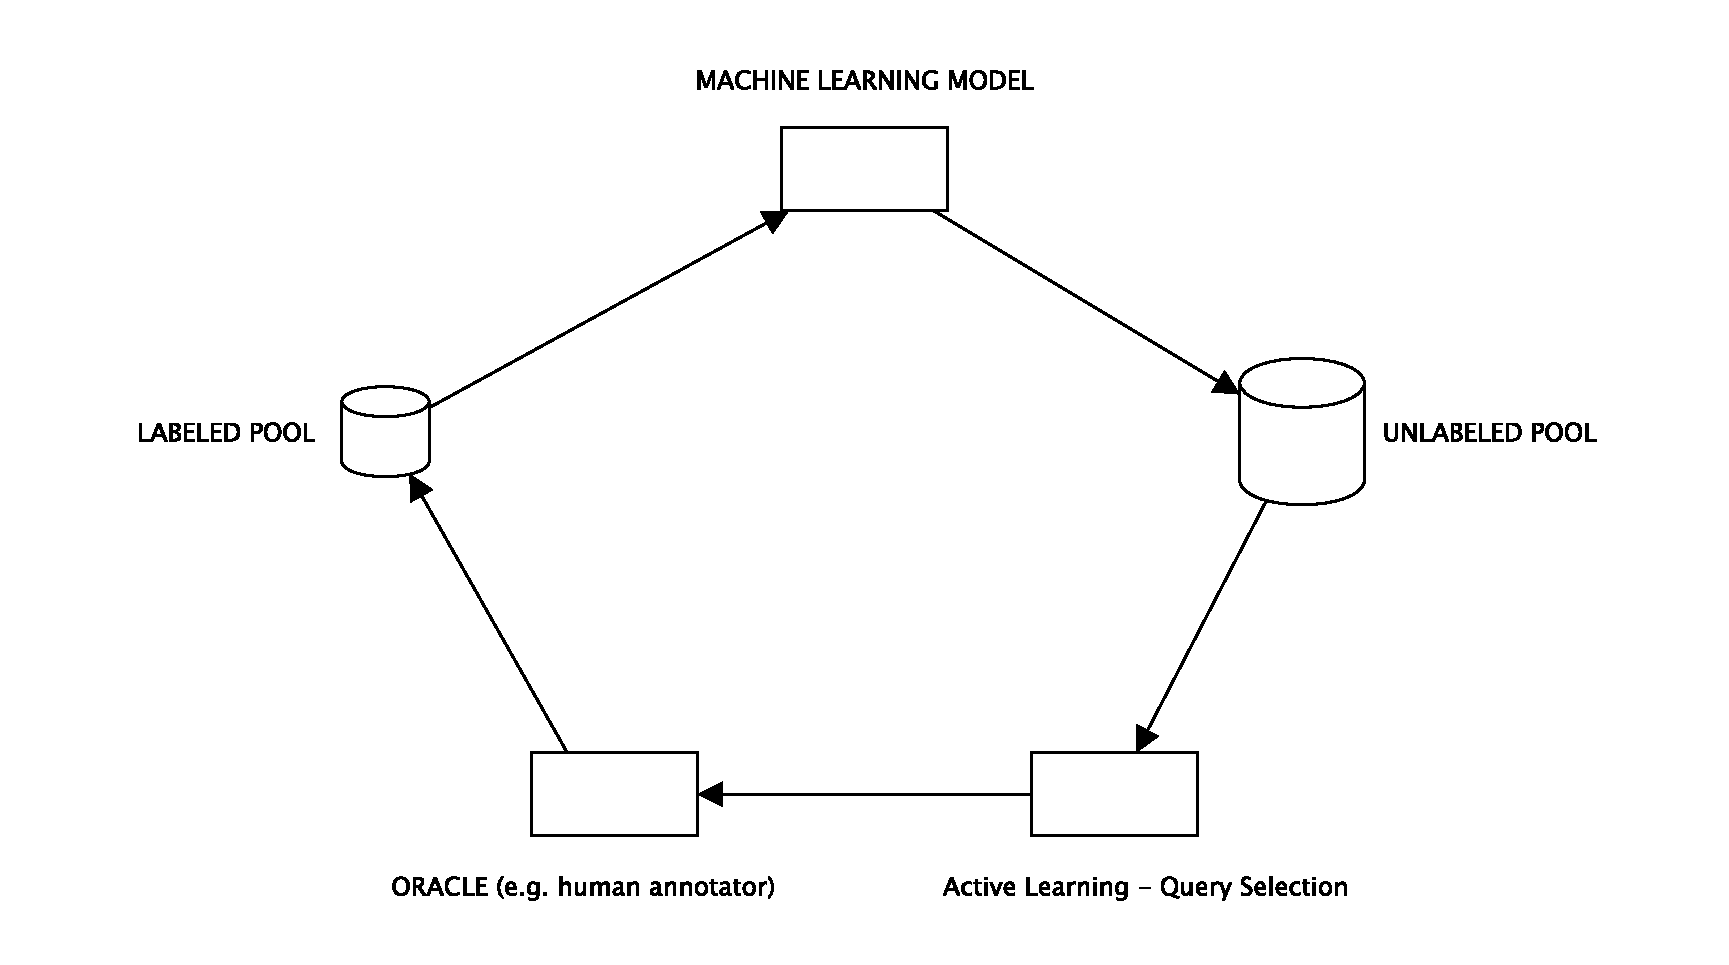
\includegraphics[width=\textwidth]{figures/active-learning-model.eps}
    \caption{An overview of an active learning system.kk}
    \label{fig:active-learning-model}
\end{figure}

If one of two categories is assigned to each document, it is called a binary classification problem~\cite{bishop2006pattern}.
Problems where one of several classes is assigned to an instance are called a multi-class classification problem.
Multi-labeled classification is when one or more categories are assigned to each document.
This thesis is mainly concerned with the multi-label case.
Assigning several categories to a document is more time consuming than in the cases where only one option needs to be identified.
In those cases the process can be stopped when the appropriate category has been found.
However, when a document can be assigned several categories, the entirety of the text needs to be considered.
For example, a news article can be on several subjects, such as both economics and sport.
Even when the category sport has already been identified, the rest of the document still has to be read in order to find any additional categories.
Using active learning to enhance the labeling of documents is therefore even more useful in the multi-labeled case, since the cost of labeling the individual reports is higher.

\section{Aim}
\label{sec:aim}

This thesis is carried out at Sectra Medical Imaging IT Solutions AB, as a part of their research division that focuses on text analytics.
The purpose with this thesis project is to evaluate different active learning techniques that can be used to increase the quato labeling  ed reports, and thereby reducing the amount of reports needed for use within the project.
Resulting from this will be a complete, standalone, system for labeling reports.
The reports are interactively queried so a user can label the ones that are deemed most useful by the system.
Labeling data to use in machine learning will probably be necessary for a long time ahead, but the aim here is to create a system that makes it more efficient.
This will then be used in conjunction with an existing web interface that Sectra created for the purpose of labeling reports.

\section{Research questions}
\label{sec:research-questions}

The specific research questions that this thesis treat are presented here.
They are the main focus of study.

\begin{enumerate}

\item \textit{To what degree is it possible to filter out invalid clinical reports by using an unsupervised techniques such as topic modeling?}
      \newline
      In the dataset from Sectra, there are reports describing patients not showing up for, or changing the time of their appointments, deceased patients or patients that have been ordered to go to another hospital.
      These reports do not contain any information of value from a medical point of view and should be discarded in the labeling process.

      Unsupervised machine learning models such as topic modeling do by definition not require any labeled documents to train on.
      If it is possible to, without any such data, to capture the necessary variance and group these invalid reports together and they can be removed from the labeling process before a doctor is presented with them.
      That would result in an additional hurdle being removed from the process.

\item \label{intro:re-q2} 
      \textit{What active learning strategies are good alternatives to sample documents at random in a multi-label document labeling system? How well do these alternatives perform?}
      \newline
      How we are choosing the documents to be sampled is important.
      If the decision boundaries of the models can be used to pick documents that would be more informative for the model, the number of labeled documents could hopefully be reduced while still obtaining the same performance.
      Another approach to selecting the documents to sample is to take advantage of the underlying structure of the data.

      The algorithms to be evaluated will be based on the models certainty, as well as taking advantage of the underlying structure of the data.
      When choosing the algorithm to use in the final system, there are several different factors that will affect the final results, and therefore need to be taken into consideration.
      How well the models perform on the data will be evaluated based on the accuracy, precision, recall and $F_1$-score of the models.
      Whether or not the algorithm needs a big initial set of labeled reports is another factor that will be evaluated.

  \item \label{intro:re-q3}
      \textit{How do the algorithms from question~\ref{intro:re-q2} affect the balance of labels in the labeled dataset?}
      Another indication on the quality of the labeled reports is the balance between the classes.
      Based on the initial sampling, the underlying distribution of labels in the clinical data is far from uniform.
      There are certain categories, like the one describing that everything is okay with the patient, that are a lot more common than other more rare illnesses.

      If the dataset that is being sampled is skewed, i.e. some categories are a more frequent than others, our labeled set will likely follow that distribution.
      This will result in models requiring a lot of labeled documents to gather a sufficient amount of reports that are of the less common categories.
      Without these, the model with only perform well on the frequently occurring categories.
      Even though the original data may be imbalanced, selecting samples that contain a better balance between the different categories could improve the performance of the models.
      When a training set is imbalanced, the standard learning algorithms' performance can be significantly reduced~\cite{he2009learning}.
      The goal here is to see which one of the different sampling techniques that will result in the best balance between the different categories in the resulting dataset.

\end{enumerate}

\section{Delimitations}
\label{sec:delimitations}

The active learning techniques will be evaluated on the publicly available Reuters dataset.
Even though the sampling strategies are evaluated objectively on this, the applicability of the techniques on clinical data is only evaluated by one physician.
This evaluation is performed on the one dataset provided by Sectra, which is not available for public use.

\section{Structure of the Report}
\label{sec:structure}

The next chapter covers the background that is relevant to understand the project.
The background is followed by the theory chapter, which brings up the theory behind the techniques used.
After this, the methodology is described, which is followed by a chapter covering the results.
The method and results are then discussed in Chapter~\ref{cha:discussion}.
Finally, Chapter~\ref{cha:conclusion} presents the conclusions.
